\phantomsection
\section*{Глава 2. Проектирование веб-приложения}
\addcontentsline{toc}{section}{Глава 2. Проектирование веб-приложения}
\stepcounter{section}
\label{sec:chapter2}

\providecommand{\tabref}[1]{\hyperref[#1]{таблице~\ref*{#1}}}
\providecommand{\figref}[1]{\hyperref[#1]{рисунке~\ref*{#1}}}

Целью данного раздела является проектирование веб-приложения до начала
непосредственной реализации программного кода. В первой главе была определена
предметная область и обоснована необходимость системы, предназначенной для
централизованного учета, хранения, анализа и синхронизации конфигурационных и
диагностических данных ПЛК LogicBox в системах АСУТП. Во второй главе
необходимо определить, кто будет пользоваться системой, какие функции она должна
предоставлять, какие данные должна хранить и по какой архитектуре будет
построена.

Основной объект разработки в рамках курсового проекта --- веб-приложение.
Локальный клиент сбора данных рассматривается только как внешний интеграционный
компонент, который передает сведения на сервер. Такой подход позволяет сохранить
фокус на дисциплине <<Разработка веб-приложений>> и одновременно учитывать
реальную специфику работы инженера АСУТП, который может находиться на объекте
без доступа к сети Интернет, но иметь доступ к локальной сети Ethernet с ПЛК.

В базовой версии проекта не предусматривается удаленное управление ПЛК через
веб-интерфейс. Система проектируется как read-mostly-среда, то есть как среда,
ориентированная преимущественно на чтение, хранение, анализ и аудит данных. Это
ограничение является принципиальным, поскольку прямое удаленное управление
промышленным оборудованием требует отдельной проработки вопросов
информационной и функциональной безопасности.

\subsection{Анализ целевой аудитории и ролей пользователей системы}

Разрабатываемое приложение предназначено для эксплуатации в инженерной среде,
связанной с сопровождением контроллеров LogicBox. В отличие от универсальных
систем хранения файлов, данное веб-приложение должно учитывать структуру
промышленного объекта, состав оборудования, историю конфигураций и ограничения
доступа пользователей к конкретным участкам АСУТП.

Под АСУТП в рамках данной работы понимается автоматизированная система
управления технологическим процессом. Под ПЛК понимается программируемый
логический контроллер, то есть устройство, исполняющее алгоритмы управления
оборудованием и взаимодействующее с датчиками, исполнительными механизмами,
панелями оператора и другими устройствами автоматизации.

\subsubsection{Целевая аудитория}

Целевая аудитория системы включает пользователей, которые участвуют в
эксплуатации, сопровождении и контроле состояния ПЛК LogicBox. Основные группы
пользователей представлены в \tabref{tab:target_audience}.

\begin{longtable}{|p{0.25\textwidth}|p{0.32\textwidth}|p{0.33\textwidth}|}
    \caption{Целевая аудитория веб-приложения} \label{tab:target_audience} \\
    \hline
    \textbf{Группа пользователей} & \textbf{Основная потребность} & \textbf{Ожидаемое использование системы} \\ \hline
    \endfirsthead

    \tabcont{\ref{tab:target_audience}}
    \textbf{Группа пользователей} & \textbf{Основная потребность} & \textbf{Ожидаемое использование системы} \\ \hline
    \endhead

    \hline
    \endfoot

    \hline
    \endlastfoot

    Инженер АСУТП & Быстро получать доступ к сведениям о разрешенных объектах, контроллерах, конфигурациях и диагностике & Просмотр карточек ПЛК, загрузка конфигураций, анализ диагностических записей, просмотр результатов синхронизации \\ \hline
    Ведущий инженер & Контролировать состояние оборудования и историю изменений в пределах закрепленных объектов & Проверка актуальности конфигураций, анализ изменений, просмотр сводной информации и результатов работы инженеров \\ \hline
    Администратор системы & Управлять пользователями, ролями, справочниками и областями доступа & Создание учетных записей, назначение ролей, настройка прав доступа к объектам эксплуатации \\ \hline
    Наблюдатель или аудитор & Получать доступ к информации без возможности изменения данных & Просмотр реестра, журналов, конфигураций, истории синхронизации и действий пользователей \\ \hline
\end{longtable}

Ключевой особенностью целевой аудитории является различие между уровнем
полномочий и областью ответственности. Один инженер может иметь право загружать
конфигурации, но только по тем объектам, которые ему назначены. Другой
пользователь может иметь доступ только на чтение, но к большему числу объектов.
Поэтому проектируемая модель доступа должна учитывать не только роль
пользователя, но и область эксплуатации, к которой он привязан.


\subsubsection{Роли пользователей}

Ролевая модель используется для разделения функций веб-приложения между разными категориями пользователей. В проектируемой системе роль определяет не конкретное место работы пользователя, а набор разрешенных действий: просмотр, создание записей, загрузку файлов, подтверждение данных, управление учетными записями и настройку доступа. При этом фактический доступ к сведениям о ПЛК дополнительно ограничивается объектами эксплуатации, назначенными пользователю.

Основные роли системы представлены в \tabref{tab:roles_permissions}.

\small
\begin{longtable}{|p{0.18\textwidth}|p{0.37\textwidth}|p{0.35\textwidth}|}
    \caption{Роли пользователей и их основные полномочия} \label{tab:roles_permissions} \\
    \hline
    \textbf{Роль} & \textbf{Назначение и разрешенные действия} & \textbf{Ограничения и особенности доступа} \\ \hline
    \endfirsthead
    \tabcont{\ref{tab:roles_permissions}}
    \textbf{Роль} & \textbf{Назначение и разрешенные действия} & \textbf{Ограничения и особенности доступа} \\ \hline
    \endhead
    \hline
    \endfoot
    \hline
    \endlastfoot

    Администратор & Обеспечивает организационную настройку системы: создает и блокирует пользователей, назначает роли, назначает области доступа, регистрирует локальные клиенты, контролирует системные журналы и справочники & Не выполняет инженерную работу с контроллерами по умолчанию. Доступ к содержимому конфигураций и диагностике предоставляется только при наличии назначенной области доступа \\ \hline

    Инженер & Выполняет основную эксплуатационную работу по закрепленным объектам: просматривает объекты эксплуатации и карточки ПЛК, добавляет и редактирует контроллеры, загружает конфигурации и файлы, просматривает диагностику и результаты синхронизации & Работает только с теми объектами эксплуатации, которые ему назначены. Не управляет пользователями, ролями и правами доступа. Не подтверждает конфигурации как проверенные или эталонные \\ \hline

    Ведущий инженер & Контролирует качество инженерных данных по закрепленным объектам: просматривает сводную аналитику, проверяет полноту карточек контроллеров, подтверждает актуальность конфигураций, контролирует результаты синхронизаций и выявляет проблемные участки & Не занимается системным администрированием пользователей. Его расширенные полномочия действуют только в пределах назначенных объектов эксплуатации или группы объектов \\ \hline

    Наблюдатель & Использует систему в режиме чтения: просматривает разрешенные объекты, карточки контроллеров, диагностические записи, файлы, отчеты и журнал синхронизации & Не создает и не изменяет записи, не загружает файлы, не подтверждает конфигурации и не управляет доступом \\ \hline

    Локальный клиент & Передает на сервер результаты локального сбора данных: сведения о найденных контроллерах, конфигурации, диагностические записи и связанные файлы & Не является пользователем-человеком и не имеет доступа к веб-интерфейсу. Работает только через серверный API и только в пределах объекта, к которому привязан при регистрации \\ \hline
\end{longtable}
\normalsize

Таким образом, инженер и ведущий инженер разделяются не формально, а по назначению выполняемых действий. Инженер наполняет систему эксплуатационными данными и работает с конкретными контроллерами. Ведущий инженер контролирует качество этих данных, подтверждает актуальность конфигураций и использует сводную аналитику для оценки состояния закрепленных объектов. Администратор отвечает за организационную и учетную часть системы, но не заменяет инженерные роли. Наблюдатель получает доступ только к просмотру данных.

Локальный клиент выделяется отдельно, поскольку он не является пользователем веб-интерфейса. Это внешний программный компонент, который проходит регистрацию на сервере и передает данные по прикладному программному интерфейсу. Прикладной программный интерфейс, или API, представляет собой набор HTTP-маршрутов и правил обмена данными между локальным клиентом и серверной частью веб-приложения.

\subsubsection{Разграничение доступа по объектам эксплуатации}

В проектируемой системе используется не только ролевая модель, но и разграничение доступа по областям ответственности. Это необходимо потому, что одна и та же роль может использоваться разными сотрудниками на разных объектах. Например, два инженера могут иметь одинаковый набор действий в системе, но один из них должен видеть только шкаф ШУ ВОМ, а другой --- только стенд LogicBox или отдельный участок АСУТП.

Доступ определяется двумя параметрами:
\begin{itemize}
    \item \textbf{роль пользователя} определяет, какие действия разрешены пользователю;
    \item \textbf{область доступа} определяет, к каким объектам эксплуатации эти действия применяются.
\end{itemize}

Областью доступа в системе является объект эксплуатации или группа объектов эксплуатации. Под объектом эксплуатации понимается площадка, шкаф, стенд, участок, АСУТП или другой логический контур, к которому привязаны контроллеры LogicBox, конфигурации, диагностические записи и файлы.

Пример применения модели доступа приведен в \tabref{tab:access_examples}.

\small
\begin{longtable}{|p{0.20\textwidth}|p{0.30\textwidth}|p{0.36\textwidth}|}
    \caption{Примеры разграничения прав по роли и области доступа} \label{tab:access_examples} \\
    \hline
    \textbf{Пользовательская роль} & \textbf{Назначенная область доступа} & \textbf{Фактически доступные действия} \\ \hline
    \endfirsthead
    \tabcont{\ref{tab:access_examples}}
    \textbf{Пользовательская роль} & \textbf{Назначенная область доступа} & \textbf{Фактически доступные действия} \\ \hline
    \endhead
    \hline
    \endfoot
    \hline
    \endlastfoot

    Инженер & ШУ ВОМ & Может вести карточки контроллеров ШУ ВОМ, загружать конфигурации и файлы, просматривать диагностику и синхронизации только по данному объекту \\ \hline
    Ведущий инженер & Участок вентиляции & Может анализировать данные по всем объектам участка, подтверждать актуальные конфигурации и контролировать полноту сведений по контроллерам участка \\ \hline
    Наблюдатель & ШУ ВОМ, стенд LogicBox & Может просматривать данные по указанным объектам, но не может изменять записи и загружать файлы \\ \hline
    Администратор & Все объекты или выбранные объекты & Может назначать пользователей на объекты и регистрировать локальные клиенты, но инженерный доступ к данным должен задаваться явно \\ \hline
    Локальный клиент & Конкретный объект эксплуатации & Может передавать на сервер данные синхронизации только по объекту, для которого был зарегистрирован \\ \hline
\end{longtable}
\normalsize

Такая модель предотвращает избыточный доступ к данным промышленной системы. Пользователь видит не весь парк ПЛК, а только те контроллеры и связанные с ними сведения, которые относятся к его зоне ответственности. В базе данных это требует хранения связей между пользователями и объектами эксплуатации, а также проверки этих связей при каждом обращении к карточке контроллера, конфигурации, диагностической записи, файлу или сессии синхронизации.

\subsection{Описание функциональности приложения}

Функциональность проектируемой системы определяется задачами, сформулированными
в первой главе, и обязательными требованиями к курсовому проекту: наличие
аутентификации и авторизации, проверки прав доступа, CRUD-интерфейса,
обработки данных, загрузки и выгрузки файлов, а также не менее трех сущностей.
В данном проекте эти требования реализуются не формально, а через предметную
задачу сопровождения ПЛК LogicBox.

CRUD --- это сокращение от Create, Read, Update, Delete, то есть создание,
чтение, изменение и удаление записей. В проектируемом приложении CRUD-интерфейс
потребуется для объектов эксплуатации, контроллеров, конфигураций,
диагностических записей, пользователей, ролей и файловых вложений.

\subsubsection{Основные функции системы}

Проектируемое веб-приложение должно предоставлять набор функций, достаточный
для централизованного ведения реестра ПЛК и связанных инженерных данных. Эти
функции сгруппированы в \tabref{tab:function_groups}.

\small
\begin{longtable}{|p{0.22\textwidth}|p{0.39\textwidth}|p{0.27\textwidth}|}
    \caption{Основные функциональные группы приложения} \label{tab:function_groups} \\
    \hline
    \textbf{Функциональная группа} & \textbf{Назначение} & \textbf{Ключевые сущности} \\ \hline
    \endfirsthead

    \tabcont{\ref{tab:function_groups}}
    \textbf{Функциональная группа} & \textbf{Назначение} & \textbf{Ключевые сущности} \\ \hline
    \endhead

    \hline
    \endfoot

    \hline
    \endlastfoot

    Аутентификация и авторизация & Вход пользователя в систему, проверка учетной записи и определение разрешенных действий & Пользователь, роль, область доступа \\ \hline
    Управление объектами эксплуатации & Ведение структуры площадок, АСУТП, шкафов и участков, в рамках которых используются ПЛК & Объект эксплуатации, пользователь \\ \hline
    Учет контроллеров & Хранение сведений о конкретных ПЛК LogicBox и их принадлежности к объектам & Контроллер, объект эксплуатации \\ \hline
    Управление конфигурациями & Хранение версий конфигураций, источников получения, дат, комментариев и признака актуальности & Конфигурация, контроллер, файл-вложение \\ \hline
    Диагностика и журналы & Хранение событий, предупреждений, ошибок и результатов локального сбора данных & Диагностическая запись, контроллер, сессия синхронизации \\ \hline
    Работа с файлами & Загрузка, скачивание и привязка файлов к сущностям системы & Файл-вложение, конфигурация, диагностика \\ \hline
    Синхронизация данных & Прием пакетов данных от локального клиента и фиксация результата обмена & Сессия синхронизации, контроллер, конфигурация, диагностика \\ \hline
    Аналитика и поиск & Фильтрация, группировка и агрегирование сведений по объектам, контроллерам, событиям и периодам & Контроллер, конфигурация, диагностическая запись \\ \hline
\end{longtable}
\normalsize

Под агрегированием данных в рамках проекта понимается объединение и группировка
записей по выбранным признакам. Например, система должна позволять определить
количество диагностических событий по объекту эксплуатации, найти контроллеры,
по которым давно не обновлялись конфигурации, или сформировать список ПЛК,
обнаруженных локальным клиентом во время конкретной сессии синхронизации.


\subsubsection{Диаграмма вариантов использования}

Диаграмма вариантов использования отражает основные действия пользователей и внешнего локального клиента. В ней отдельно выделены администратор, инженер, ведущий инженер, наблюдатель и локальный клиент. Такое разделение необходимо, поскольку инженер и ведущий инженер выполняют разные задачи: инженер наполняет систему эксплуатационными данными, а ведущий инженер контролирует их актуальность, полноту и качество.

Диаграмма приведена на \figref{fig:usecase2}.

\begin{figure}[H]
    \centering
    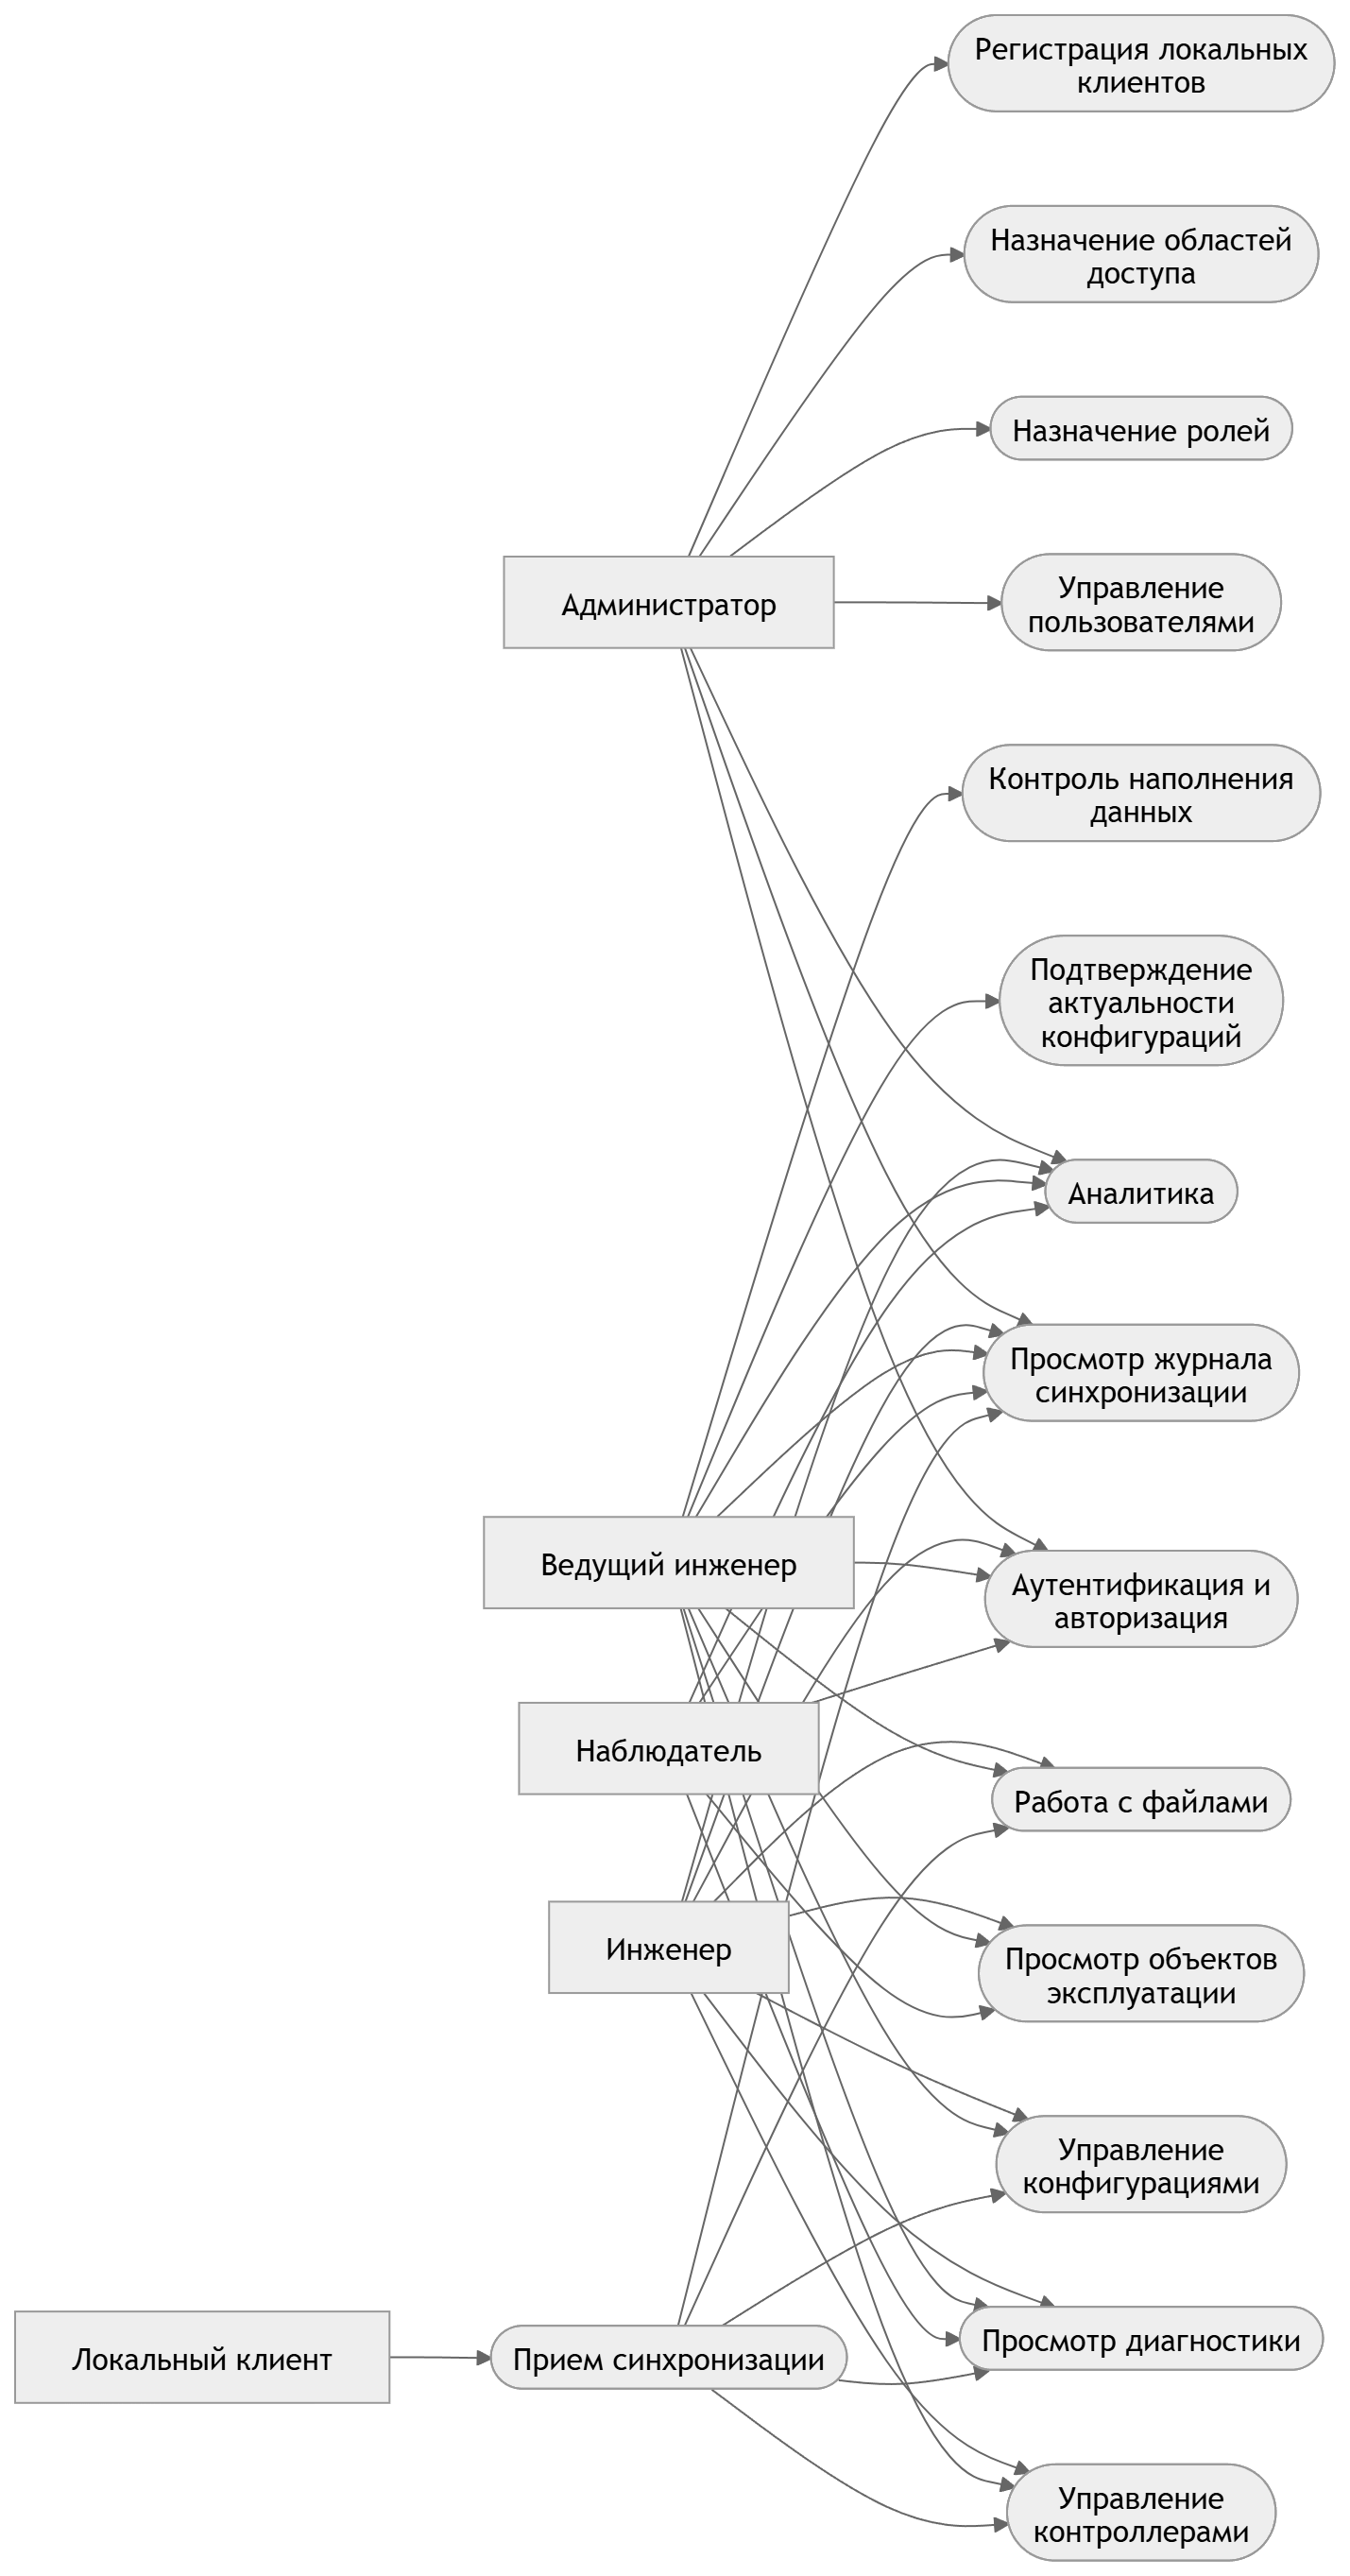
\includegraphics[width=0.90\textwidth,height=0.70\textheight,keepaspectratio]{images/diagrams/use_case.png}
    \caption{Диаграмма вариантов использования проектируемой системы}
    \label{fig:usecase2}
\end{figure}

Администратор выполняет функции настройки системы: управляет пользователями, назначает роли, назначает области доступа и регистрирует локальные клиенты. Инженер работает с эксплуатационными данными по закрепленным объектам: объектами эксплуатации, контроллерами, конфигурациями, диагностикой, файлами и результатами синхронизации. Ведущий инженер дополнительно выполняет контрольные функции: подтверждает актуальность конфигураций, проверяет полноту наполнения карточек контроллеров и анализирует состояние объектов. Наблюдатель имеет только функции просмотра. Локальный клиент участвует только в сценарии передачи данных на сервер и не получает доступа к пользовательскому интерфейсу.

\subsubsection{User story}

Для уточнения ожидаемого поведения системы были сформулированы типовые пользовательские истории:
\begin{itemize}
    \item как администратор, я хочу создавать пользователей, назначать им роли и области доступа, чтобы каждый сотрудник работал только с теми объектами, за которые он отвечает;
    \item как администратор, я хочу регистрировать локальные клиенты и привязывать их к конкретным объектам эксплуатации, чтобы данные синхронизации не попадали в систему без контроля источника;
    \item как инженер, я хочу видеть список только закрепленных за мной объектов эксплуатации, чтобы работать с нужными ПЛК без доступа к чужим промышленным данным;
    \item как инженер, я хочу вести карточки контроллеров, загружать конфигурации, журналы и файлы, чтобы фиксировать результаты сопровождения оборудования;
    \item как инженер, я хочу просматривать диагностические записи с фильтрами по объекту, ПЛК, уровню события и периоду, чтобы быстрее находить проблемы в работе оборудования;
    \item как ведущий инженер, я хочу видеть сводную аналитику по закрепленным объектам, чтобы оценивать состояние контроллеров, частоту диагностических событий и результаты синхронизаций;
    \item как ведущий инженер, я хочу подтверждать актуальность выбранной конфигурации контроллера, чтобы в системе было понятно, какая версия считается проверенной и рабочей;
    \item как ведущий инженер, я хочу контролировать полноту карточек ПЛК и наличие связанных файлов, чтобы база не превращалась в набор разрозненных записей;
    \item как наблюдатель, я хочу просматривать разрешенные объекты, диагностику, файлы и журнал синхронизации без права изменения, чтобы использовать систему для контроля и аудита;
    \item как локальный клиент, я хочу передавать на сервер результаты локального сбора данных по привязанному объекту, чтобы данные, полученные инженером на объекте без доступа к Интернету, затем попадали в общую базу.
\end{itemize}

\subsubsection{Сценарии работы пользователей}

Ключевые сценарии работы системы можно представить следующим образом.

\textbf{Сценарий 1. Настройка пользователей, ролей и областей доступа.} Администратор входит в систему, открывает раздел управления пользователями, создает или редактирует учетную запись сотрудника, назначает ему роль и указывает область доступа. Например, инженеру назначается роль инженера и объект эксплуатации ШУ ВОМ, а ведущему инженеру назначается участок вентиляции, включающий несколько шкафов. После сохранения настроек пользователь получает доступ только к тем функциям и данным, которые соответствуют его роли и области ответственности.

\textbf{Сценарий 2. Регистрация локального клиента.} Администратор открывает раздел синхронизации и регистрирует локальный клиент, который будет использоваться на ноутбуке инженера. При регистрации задаются имя клиента, ответственный пользователь и объект эксплуатации, по которому клиент имеет право передавать данные. В результате сервер формирует отдельные учетные данные для клиента. Это позволяет принимать данные синхронизации без хранения пароля пользователя в локальной программе.

\textbf{Сценарий 3. Работа инженера с контроллерами и конфигурациями.} Инженер проходит аутентификацию и видит только закрепленные за ним объекты эксплуатации. После выбора объекта он открывает список контроллеров, переходит в карточку ПЛК, проверяет основные сведения, загружает новую конфигурацию или связанный файл. Сервер проверяет право доступа к объекту, сохраняет метаданные в базе данных, а файл размещает в файловом хранилище.

\textbf{Сценарий 4. Анализ диагностических записей инженером.} Инженер открывает журнал диагностики, выбирает объект эксплуатации, контроллер, уровень события и период. Система возвращает только те диагностические записи, которые относятся к разрешенным объектам. По результатам просмотра инженер может открыть карточку контроллера, скачать связанный файл или сравнить диагностические события с историей конфигураций.

\textbf{Сценарий 5. Контроль данных ведущим инженером.} Ведущий инженер открывает панель аналитики по закрепленному участку или группе объектов. Система показывает сводные сведения о контроллерах, количестве диагностических событий, последних синхронизациях и конфигурациях, ожидающих проверки. После проверки ведущий инженер может отметить выбранную конфигурацию как актуальную, оставить комментарий и тем самым зафиксировать проверенную версию данных.

\textbf{Сценарий 6. Контроль полноты наполнения ведущим инженером.} Ведущий инженер просматривает список контроллеров, у которых отсутствуют актуальные конфигурации, вложенные файлы или свежие данные синхронизации. Такие записи требуют дополнительной проверки инженером. В результате система используется не только как хранилище, но и как инструмент контроля качества эксплуатационных данных.

\textbf{Сценарий 7. Просмотр данных наблюдателем.} Наблюдатель входит в систему и получает доступ к страницам просмотра разрешенных объектов, карточек контроллеров, диагностических записей, файлов и сессий синхронизации. При попытке выполнить изменение, загрузку файла или подтверждение конфигурации система должна отказать в выполнении операции, так как роль наблюдателя не содержит соответствующих прав.

\textbf{Сценарий 8. Прием данных от локального клиента.} Локальный клиент собирает сведения о контроллерах в локальной сети объекта и формирует пакет синхронизации. При подключении к серверу клиент передает пакет по API. Сервер проверяет подлинность клиента и его привязку к объекту эксплуатации, создает запись сессии синхронизации, сохраняет контроллеры, конфигурации, диагностические записи и файлы. После обработки данные становятся доступны инженеру и ведущему инженеру в пределах их областей доступа.

Перечисленные сценарии показывают, что система не ограничивается простой загрузкой файлов. Она связывает роли пользователей, области доступа, карточки контроллеров, конфигурации, диагностику, файлы и сессии синхронизации в единую модель сопровождения ПЛК LogicBox.

\subsection{Проектирование модели данных}

Модель данных должна отражать предметную область и обеспечивать реализацию
основных функций приложения. В проектируемой системе данные группируются вокруг
контроллера LogicBox, который связан с объектом эксплуатации, конфигурациями,
диагностическими записями, файлами и сессиями синхронизации.

\subsubsection{Состав основных сущностей}

Основные сущности проектируемой системы приведены в \tabref{tab:entities}. В
таблице указано не только название сущности, но и ее назначение в приложении.

\small
\begin{longtable}{|p{0.22\textwidth}|p{0.38\textwidth}|p{0.28\textwidth}|}
    \caption{Основные сущности предметной модели} \label{tab:entities} \\
    \hline
    \textbf{Сущность} & \textbf{Назначение} & \textbf{Пример ключевых атрибутов} \\ \hline
    \endfirsthead

    \tabcont{\ref{tab:entities}}
    \textbf{Сущность} & \textbf{Назначение} & \textbf{Пример ключевых атрибутов} \\ \hline
    \endhead

    \hline
    \endfoot

    \hline
    \endlastfoot

    Пользователь & Описывает человека, работающего с системой, и используется для аутентификации, авторизации и аудита действий & id, ФИО, email, password\_hash, status, created\_at \\ \hline
    Роль & Определяет набор допустимых действий пользователя в системе & id, name, description, permissions \\ \hline
    Объект эксплуатации & Описывает площадку, АСУТП, шкаф или участок, к которому относятся контроллеры & id, name, type, location, description, status \\ \hline
    Контроллер & Описывает конкретный ПЛК LogicBox и связывает с ним конфигурации, диагностику и файлы & id, object\_id, name, ip\_address, mac\_address, model, firmware\_version, last\_seen\_at \\ \hline
    Конфигурация & Хранит версию конфигурационных данных контроллера и сведения об источнике получения & id, controller\_id, version, source, checksum, is\_actual, created\_at \\ \hline
    Диагностическая запись & Фиксирует событие, ошибку, предупреждение или результат проверки ПЛК & id, controller\_id, level, event\_type, message, occurred\_at, status \\ \hline
    Файл-вложение & Хранит метаданные загруженного файла и его связь с объектами системы & id, owner\_type, owner\_id, file\_name, storage\_path, size, checksum \\ \hline
    Сессия синхронизации & Описывает факт передачи данных от локального клиента на сервер & id, user\_id, device\_name, started\_at, finished\_at, status, records\_count \\ \hline
\end{longtable}
\normalsize

Сущность <<Пользователь>> необходима для привязки действий к конкретному
человеку. Сущность <<Роль>> задает общий уровень полномочий. Сущность <<Объект
эксплуатации>> ограничивает область доступа и связывает данные с реальным
промышленным контекстом. Сущность <<Контроллер>> является центральной сущностью
модели, поскольку именно вокруг конкретного ПЛК накапливаются конфигурации,
диагностика и файлы. Сущность <<Сессия синхронизации>> нужна для контроля
передачи данных от внешнего локального клиента и предотвращения потери истории
обмена.

\subsubsection{ER-диаграмма}

ER-диаграмма отражает связи между сущностями предметной области. ER означает
Entity--Relationship, то есть <<сущность--связь>>. Диаграмма показывает, какие
таблицы будут существовать в базе данных и как они будут связаны между собой.
Упрощенное представление ER-модели приведено на \figref{fig:er_model}.

\begin{figure}[ht!]
    \centering
    \fbox{%
    \begin{minipage}{0.92\textwidth}
        \centering
        \textbf{ER-модель проектируемой системы}\\[6pt]
        \begin{tabularx}{0.90\textwidth}{|p{0.28\textwidth}|X|}
            \hline
            User $\leftrightarrow$ Role & Пользователь имеет одну или несколько ролей; роль может быть назначена нескольким пользователям \\ \hline
            User $\leftrightarrow$ Object & Пользователь получает доступ к одному или нескольким объектам эксплуатации через таблицу назначений доступа \\ \hline
            Object $\rightarrow$ Controller & Один объект эксплуатации может содержать несколько контроллеров \\ \hline
            Controller $\rightarrow$ Configuration & Один контроллер может иметь несколько версий конфигураций \\ \hline
            Controller $\rightarrow$ DiagnosticRecord & Один контроллер может иметь несколько диагностических записей \\ \hline
            SyncSession $\rightarrow$ Controller & Одна сессия синхронизации может включать данные по нескольким контроллерам \\ \hline
            Attachment $\rightarrow$ Entity & Файл-вложение может быть связан с конфигурацией, диагностической записью, контроллером или сессией синхронизации \\ \hline
        \end{tabularx}
    \end{minipage}}
    \caption{Упрощенная ER-модель веб-приложения}
    \label{fig:er_model}
\end{figure}

Для реализации связи пользователя с объектами эксплуатации требуется отдельная
таблица назначений доступа. Она позволяет назначить одному пользователю доступ к
нескольким объектам и одновременно назначить один объект нескольким
пользователям. Аналогично для ролей может использоваться связующая таблица,
если пользователю допускается назначать более одной роли.

\subsubsection{Логическая схема базы данных}

Логическая схема базы данных определяет состав таблиц, связи между ними и
ключевые ограничения. На уровне проектирования выделяются следующие таблицы:
\texttt{users}, \texttt{roles}, \texttt{user\_roles},
\texttt{operation\_objects}, \texttt{user\_object\_access},
\texttt{controllers}, \texttt{configurations}, \texttt{diagnostic\_records},
\texttt{attachments}, \texttt{sync\_sessions} и
\texttt{sync\_session\_items}.

Назначение основных таблиц логической схемы приведено в
\tabref{tab:logical_schema}.

\small
\begin{longtable}{|p{0.25\textwidth}|p{0.36\textwidth}|p{0.27\textwidth}|}
    \caption{Логическая схема базы данных} \label{tab:logical_schema} \\
    \hline
    \textbf{Таблица} & \textbf{Назначение} & \textbf{Основные связи} \\ \hline
    \endfirsthead

    \tabcont{\ref{tab:logical_schema}}
    \textbf{Таблица} & \textbf{Назначение} & \textbf{Основные связи} \\ \hline
    \endhead

    \hline
    \endfoot

    \hline
    \endlastfoot

    \texttt{users} & Хранение учетных записей пользователей & Связь с ролями, объектами доступа, сессиями синхронизации и загруженными файлами \\ \hline
    \texttt{roles} & Хранение ролей и набора разрешений & Связь с пользователями через \texttt{user\_roles} \\ \hline
    \texttt{operation\_objects} & Хранение объектов эксплуатации: площадок, АСУТП, шкафов или участков & Связь с контроллерами и назначениями доступа \\ \hline
    \texttt{controllers} & Хранение данных о ПЛК LogicBox & Связь с объектом эксплуатации, конфигурациями, диагностикой и файлами \\ \hline
    \texttt{configurations} & Хранение версий конфигураций контроллеров & Связь с контроллером, пользователем, сессией синхронизации и вложениями \\ \hline
    \texttt{diagnostic\_records} & Хранение диагностических событий и сообщений & Связь с контроллером, объектом эксплуатации и сессией синхронизации \\ \hline
    \texttt{attachments} & Хранение метаданных файлов & Полиморфная связь с разными сущностями через \texttt{owner\_type} и \texttt{owner\_id} \\ \hline
    \texttt{sync\_sessions} & Хранение фактов обмена данными между локальным клиентом и сервером & Связь с пользователем, локальным устройством, полученными данными и файлами \\ \hline
\end{longtable}
\normalsize

Файлы конфигураций, архивы и журналы нецелесообразно хранить непосредственно в
таблицах базы данных в виде крупных бинарных полей. В проектируемой архитектуре
в базе данных хранятся метаданные файла: имя, тип, размер, контрольная сумма,
путь в файловом хранилище и связь с предметной сущностью. Сам файл хранится в
каталоге файлового хранилища сервера. Такой подход упрощает резервное
копирование, скачивание файлов и контроль целостности.

\subsubsection{Физическая схема базы данных}

На физическом уровне в качестве системы управления базами данных планируется
использовать PostgreSQL. Эта СУБД подходит для веб-приложений с реляционной
структурой данных, поддерживает внешние ключи, индексы, транзакции и достаточно
гибкую работу с датами, текстовыми полями и JSON-данными. JSON-поля могут быть
полезны для хранения части технических сведений, полученных от локального
клиента, если состав этих сведений может изменяться между версиями утилит.

Для обеспечения производительности и удобства поиска предусматриваются индексы:
\begin{itemize}
    \item по внешним ключам, связывающим контроллеры, конфигурации и диагностику;
    \item по IP-адресу и MAC-адресу контроллера;
    \item по дате диагностического события;
    \item по статусу и времени сессии синхронизации;
    \item по признаку актуальности конфигурации.
\end{itemize}

Отдельное внимание уделяется ограничению целостности. Например, конфигурация не
может существовать без контроллера, диагностическая запись должна быть связана с
контроллером, а доступ пользователя к объекту эксплуатации должен ссылаться на
существующую учетную запись и существующий объект. Такая структура уменьшает
риск появления несвязанных данных, которые невозможно интерпретировать в
инженерном контексте.

\subsection{Проектирование архитектуры интерфейсов, загрузки и выгрузки файлов, а также макетов страниц}

Архитектура приложения должна обеспечивать разделение пользовательского
интерфейса, серверной логики, доступа к данным и интеграции с локальным
клиентом. Такое разделение необходимо для сопровождения проекта, тестирования и
возможной замены конкретного серверного стека без переработки всей предметной
модели.

\subsubsection{Обоснование выбора технологического стека}

В качестве основного серверного стека выбран язык Go и веб-фреймворк Fiber. Go
является компилируемым языком со статической типизацией. Статическая типизация
позволяет выявлять часть ошибок на этапе сборки, что важно для приложения,
работающего с правами доступа, файлами и связанными данными. Компиляция в один
исполняемый файл упрощает развертывание серверной части: для запуска приложения
не требуется переносить большое количество интерпретируемых зависимостей.

Fiber выбран как легковесный веб-фреймворк для Go, позволяющий реализовать
маршрутизацию, middleware, обработку HTTP-запросов, работу со статическими
файлами и шаблонами. Middleware --- это промежуточный обработчик запроса,
который выполняется между получением HTTP-запроса и вызовом конкретного
обработчика маршрута. В проектируемой системе middleware может использоваться
для проверки сессии пользователя, роли, области доступа и журналирования
операций.

Распространенной альтернативой для учебных веб-приложений является связка
Python и Flask. Flask также подходит для разработки приложений подобного класса:
он прост в изучении, имеет развитую экосистему и позволяет быстро создавать
маршруты и шаблоны. Выбор Go и Fiber в данном проекте не означает непригодность
Flask. Он обусловлен тем, что Go хорошо подходит для разработки серверных
приложений с HTTP API, файловыми операциями, обработкой структурированных
данных и потенциальной интеграцией с внешними утилитами. Кроме того, наличие
практического опыта разработки на Go снижает проектные риски и повышает
вероятность завершения рабочей реализации в ограниченные сроки курсового
проекта.

Сравнение выбранного стека с альтернативным вариантом приведено в
\tabref{tab:stack_compare}.

\small
\begin{longtable}{|p{0.22\textwidth}|p{0.30\textwidth}|p{0.34\textwidth}|}
    \caption{Сравнение вариантов серверного стека} \label{tab:stack_compare} \\
    \hline
    \textbf{Критерий} & \textbf{Go + Fiber} & \textbf{Python + Flask} \\ \hline
    \endfirsthead

    \tabcont{\ref{tab:stack_compare}}
    \textbf{Критерий} & \textbf{Go + Fiber} & \textbf{Python + Flask} \\ \hline
    \endhead

    \hline
    \endfoot

    \hline
    \endlastfoot

    Типизация & Статическая типизация, часть ошибок выявляется при сборке & Динамическая типизация, выше требования к тестированию и дисциплине разработки \\ \hline
    Развертывание & Возможность сборки в один исполняемый файл & Требуется окружение Python и установка зависимостей \\ \hline
    Работа с HTTP API & Хорошо подходит для реализации REST-подобного API и middleware & Также хорошо подходит для API и веб-страниц \\ \hline
    Поддержка шаблонов & Возможна серверная генерация HTML-страниц & Возможна серверная генерация HTML-страниц \\ \hline
    Проектный риск & Ниже за счет имеющегося опыта разработки на Go & Выше, если язык и экосистема требуют дополнительного изучения \\ \hline
    Заменяемость в архитектуре & Реализация может быть заменена при сохранении схемы БД, HTTP API и HTML-макетов & Может быть альтернативной реализацией той же архитектуры \\ \hline
\end{longtable}
\normalsize

Для клиентской части выбран базовый стек HTML, CSS и JavaScript. HTML задает
структуру страниц, CSS отвечает за визуальное оформление, а JavaScript
используется для интерактивных элементов: фильтров, раскрывающихся блоков,
проверки форм и динамического обновления отдельных элементов интерфейса. В
рамках проектируемого приложения основной интерфейс состоит из форм, таблиц,
карточек и фильтров, поэтому применение тяжелого SPA-фреймворка не является
обязательным. SPA, или single-page application, --- это одностраничное
приложение, в котором большая часть логики интерфейса выполняется на клиентской
стороне. Для данного проекта такой подход может избыточно усложнить реализацию.

Использование HTML-макетов во втором разделе имеет практическое преимущество:
эти макеты могут стать основой реальных шаблонов страниц в третьем разделе.
Таким образом, проектирование интерфейсов не сводится к статическим картинкам,
а сразу формирует заготовки будущего веб-приложения.

\subsubsection{Архитектурная независимость от конкретного backend-стека}

Несмотря на выбор Go и Fiber, архитектура проектируется так, чтобы основные
решения не зависели жестко от конкретного фреймворка. Это означает, что при
необходимости серверная реализация может быть перенесена, например, на Python и
Flask без полной переработки предметной модели, структуры базы данных и
пользовательских сценариев.

Для достижения такой независимости приложение делится на логические слои:
\begin{itemize}
    \item слой представления, отвечающий за HTML-страницы, формы, таблицы и пользовательские действия;
    \item прикладной слой, содержащий сценарии работы системы: создание контроллера, загрузка конфигурации, прием данных синхронизации;
    \item слой доступа к данным, отвечающий за работу с базой данных и файловым хранилищем;
    \item интеграционный слой, отвечающий за API для локального клиента.
\end{itemize}

При такой организации маршруты Fiber, обработчики HTTP-запросов и шаблонизатор
не должны содержать всю бизнес-логику. Они должны принимать запрос, выполнять
проверку пользователя и передавать управление прикладным сервисам. Предметные
сущности, правила доступа, схема базы данных и API-контракты остаются
независимыми от конкретной технологии реализации серверной части.

\subsubsection{Логическая архитектура веб-приложения}

Логическая архитектура приложения включает веб-интерфейс, серверную часть, базу
данных, файловое хранилище и внешний локальный клиент. Общий вид архитектуры
представлен на \figref{fig:logical_architecture}.

\begin{figure}[ht!]
    \centering
    \fbox{%
    \begin{minipage}{0.92\textwidth}
        \centering
        \textbf{Логическая архитектура}\\[8pt]
        \begin{tabularx}{0.88\textwidth}{|p{0.25\textwidth}|X|}
            \hline
            Веб-интерфейс & HTML-страницы, формы, таблицы, фильтры, карточки объектов и контроллеров \\ \hline
            Backend & Аутентификация, авторизация, CRUD, бизнес-правила, обработка файлов, API синхронизации \\ \hline
            База данных & Пользователи, роли, объекты эксплуатации, контроллеры, конфигурации, диагностика, сессии синхронизации \\ \hline
            Файловое хранилище & Конфигурационные файлы, журналы, архивы, отчеты и вложения \\ \hline
            Локальный клиент & Внешний компонент, который собирает данные в локальной сети объекта и передает их на сервер \\ \hline
        \end{tabularx}
    \end{minipage}}
    \caption{Логическая архитектура веб-приложения}
    \label{fig:logical_architecture}
\end{figure}

Серверная часть содержит следующие основные модули:
\begin{itemize}
    \item модуль аутентификации и управления пользовательскими сессиями;
    \item модуль авторизации и проверки доступа к объектам эксплуатации;
    \item модуль управления объектами и контроллерами;
    \item модуль конфигураций и версий;
    \item модуль диагностических записей;
    \item модуль файловых вложений;
    \item модуль приема данных от локального клиента;
    \item модуль поиска, фильтрации и агрегирования данных.
\end{itemize}

Такое разбиение упрощает дальнейшую реализацию: каждый модуль может быть
разработан и протестирован отдельно, а изменения в интерфейсе не требуют
переписывания логики хранения данных.

\subsubsection{Архитектура загрузки и выгрузки файлов}

Загрузка и выгрузка файлов является обязательной частью проекта и одновременно
важной предметной функцией. В системе предполагается хранить файлы конфигураций,
журналы, архивы, результаты выгрузок, комментарии и иные материалы, связанные с
контроллерами LogicBox.

При загрузке файла сервер должен выполнить следующие действия:
\begin{enumerate}
    \item проверить, что пользователь аутентифицирован;
    \item проверить, что пользователь имеет право загружать файлы для выбранного объекта или контроллера;
    \item проверить тип и размер файла;
    \item сохранить файл в файловом хранилище;
    \item записать метаданные файла в таблицу \texttt{attachments};
    \item связать файл с конфигурацией, диагностической записью, контроллером или сессией синхронизации;
    \item зафиксировать автора и время загрузки.
\end{enumerate}

При скачивании файла сервер также не должен отдавать файл только по прямому
пути. Пользователь сначала обращается к маршруту веб-приложения, сервер
проверяет его права на связанную сущность и только после этого возвращает файл.
Такой подход позволяет не раскрывать внутреннюю структуру файлового хранилища и
не допускать скачивания материалов по случайно полученной ссылке.

\subsubsection{Взаимодействие сервера с локальным клиентом}

Локальный клиент в рамках данного проекта не является самостоятельным предметом
разработки, но его взаимодействие с веб-приложением должно быть спроектировано.
Это необходимо для того, чтобы серверная часть заранее учитывала прием данных,
собранных на объекте без постоянного доступа к Интернету.

Сценарий взаимодействия выглядит следующим образом:
\begin{enumerate}
    \item инженер запускает локальный клиент на ноутбуке в сети объекта;
    \item клиент собирает сведения о доступных ПЛК LogicBox и сохраняет их локально;
    \item при появлении связи с сервером клиент отправляет пакет данных через API;
    \item сервер проверяет токен клиента и область доступа пользователя;
    \item сервер создает сессию синхронизации;
    \item сервер сохраняет сведения о контроллерах, конфигурациях, диагностике и файлах;
    \item результат синхронизации отображается в веб-интерфейсе.
\end{enumerate}

На стороне веб-приложения достаточно спроектировать API приема данных и страницу
просмотра сессий синхронизации. Внутренняя реализация локального клиента может
развиваться отдельно. При этом API-контракт должен быть стабильным: клиент
передает идентификатор устройства, сведения о пользователе или токене,
метаданные объекта эксплуатации, список найденных контроллеров, конфигурации,
диагностические записи и вложения.

\subsubsection{Макеты основных страниц}

Макеты страниц выполняются в виде HTML-документов, поскольку в дальнейшем они
могут быть использованы как основа реальных шаблонов веб-приложения. Такой
подход уменьшает объем повторной работы: созданные во втором разделе макеты не
остаются только изображениями, а становятся заготовкой интерфейса для третьего
раздела.

Минимальный набор проектируемых страниц приведен в \tabref{tab:page_mockups}.

\small
\begin{longtable}{|p{0.24\textwidth}|p{0.38\textwidth}|p{0.26\textwidth}|}
    \caption{Макеты основных страниц веб-приложения} \label{tab:page_mockups} \\
    \hline
    \textbf{Страница} & \textbf{Назначение} & \textbf{Основные элементы} \\ \hline
    \endfirsthead

    \tabcont{\ref{tab:page_mockups}}
    \textbf{Страница} & \textbf{Назначение} & \textbf{Основные элементы} \\ \hline
    \endhead

    \hline
    \endfoot

    \hline
    \endlastfoot

    Страница входа & Аутентификация пользователя & Логин, пароль, кнопка входа, сообщение об ошибке \\ \hline
    Панель управления & Быстрый обзор разрешенных объектов и состояния системы & Карточки показателей, последние события, последние синхронизации \\ \hline
    Список объектов эксплуатации & Просмотр объектов, доступных пользователю & Таблица объектов, поиск, фильтр, кнопка добавления \\ \hline
    Список контроллеров & Просмотр ПЛК в рамках выбранного объекта & Таблица ПЛК, статус, IP-адрес, последняя синхронизация \\ \hline
    Карточка контроллера & Детальный просмотр сведений о ПЛК & Основные параметры, конфигурации, диагностика, файлы \\ \hline
    Диагностика & Анализ событий и ошибок & Фильтры по датам, объектам, уровню важности и типу события \\ \hline
    Сессии синхронизации & Просмотр результатов обмена с локальным клиентом & Статус, время, источник, количество записей, ошибки \\ \hline
    Пользователи и роли & Администрирование доступа & Список пользователей, роли, области доступа, статус учетной записи \\ \hline
\end{longtable}
\normalsize

Упрощенное представление структуры ключевых страниц показано на
\figref{fig:mockups}. В реальной реализации эти макеты будут оформлены как
HTML-страницы с общим CSS-файлом и минимальным JavaScript для фильтров,
раскрытия блоков и проверки форм.

\begin{figure}[ht!]
    \centering
    \fbox{%
    \begin{minipage}{0.92\textwidth}
        \textbf{Панель управления}\\
        Верхнее меню: объекты, контроллеры, диагностика, синхронизация, администрирование.\\
        Карточки: количество объектов, количество ПЛК, события за период, последняя синхронизация.\\[6pt]
        \textbf{Карточка контроллера}\\
        Блок параметров: имя, объект, IP, MAC, модель, прошивка, статус.\\
        Вкладки: конфигурации, диагностика, файлы, история синхронизации.\\[6pt]
        \textbf{Диагностика}\\
        Фильтры: объект, контроллер, период, уровень, тип события. Ниже --- таблица записей и сводка.\\[6pt]
        \textbf{Сессии синхронизации}\\
        Таблица сессий: дата, локальный клиент, объект, статус, количество записей, ошибки.
    \end{minipage}}
    \caption{Упрощенные макеты основных страниц веб-приложения}
    \label{fig:mockups}
\end{figure}

При дальнейшей разработке на основе этих макетов будут подготовлены HTML-шаблоны
для серверной генерации страниц. Это соответствует выбранной архитектуре:
сервер формирует страницы и передает пользователю готовый HTML, а JavaScript
используется точечно для повышения удобства работы, не превращая приложение в
избыточно сложную одностраничную систему.

